\documentclass[10pt,a4paper, margin=1in]{article}
\usepackage{fullpage}
\usepackage{amsfonts, amsmath, pifont}
\usepackage{amsthm}
\usepackage{graphicx}
\usepackage{pgfplots}
\usepackage{tikz}
\usepackage{float}
\usepackage{tkz-euclide}
\pgfplotsset{compat=1.13}


\usetikzlibrary{angles,quotes}

\DeclareMathOperator{\taninv}{\tan^{-1}}

\begin{filecontents}{q4a_1.dat}
 n   xn
 -7  -4
 -6   0
 -5   0  
 -4   3
 -3   0
 -2  -2 
 -1   0
 0    0
 1    1
 2 	  0
 3    0
 4    0
 5    0
 6    0
 7    0
\end{filecontents}

\begin{filecontents}{q4a_2.dat}
 n   xn
 -1    1
 0	   0
 1     0
 2     0
 3     -4
 4     0
 5     0
 6     0
 7     0
\end{filecontents}

\begin{filecontents}{q4a_3.dat}
 n   xn
 -7   -4
 -6    0
 -5    0
 -4    3
 -3    0
 -2    -2
 -1    1
 0	   0
 1     1
 2     0
 3     -4
 4     0
 5     0
 6     0
 7     0
\end{filecontents}


\usepackage{geometry}
 \geometry{
 a4paper,
 total={210mm,297mm},
 left=10mm,
 right=10mm,
 top=10mm,
 bottom=10mm,
 }
 % Write both of your names here. Fill exxxxxxx with your ceng mail address.
 \author{
  TONKAL, Özlem\\
  \texttt{e1881531@ceng.metu.edu.tr}
  \and
  BAŞŞİMŞEK, Orçun\\
  \texttt{e2098804@ceng.metu.edu.tr}
}
\title{CENG 384 - Signals and Systems for Computer Engineers \\
Spring 2021 \\
Homework 1}
\begin{document}
\maketitle



\noindent\rule{19cm}{1.2pt}

\begin{enumerate}

\item %write the solution of q1
In the lectures, we have seen that: \\
\[ e^t = \sum_{k=0}^{\infty} \frac{t^k}{k!} \]
\\
If we expand this summation:

$e^t = \frac{t^0}{0!} + \frac{t^1}{1!} + \frac{t^2}{2!} + \frac{t^3}{3!} + \frac{t^4}{4!} + \frac{t^5}{5!} + \frac{t^6}{6!} + ...$ \\
\\
$e^t = 1 + \frac{t}{1!} + \frac{t^2}{2!} + \frac{t^3}{3!} + \frac{t^4}{4!} + \frac{t^5}{5!} + \frac{t^6}{6!} + ...$
\\
\\
If we take derivative of both side:
\\
$\frac{de^t}{dt} = \frac{d}{dt}(1 + \frac{t}{1!} + \frac{t^2}{2!} + \frac{t^3}{3!} + \frac{t^4}{4!} + \frac{t^5}{5!} + \frac{t^6}{6!} + ...)$ \\
\\
$\frac{de^t}{dt} = 0 + \frac{1}{1!} + \frac{2t}{2!} + \frac{3t^2}{3!} + \frac{4t^3}{4!} + \frac{5t^4}{5!} + \frac{6t^5}{6!} + ...$ \\
\\
$\frac{de^t}{dt} = 1 + \frac{t}{1!} + \frac{t^2}{2!} + \frac{t^3}{3!} + \frac{t^4}{4!} + \frac{t^5}{5!} + ... = e^t$
\\
As you see, after simplifying the right hand side, we reached the same $e^t$ according to above definition since it goes to infinity. \\
Therefore, $\frac{de^t}{dt} = e^t$

\item %write the solution of q2
    \begin{enumerate}
    % Write your solutions in the following items.
    \item %write the solution of q2a
    If $z = x +jy$ \ and \ $z-3 = j -2\bar{z}$ and, we also know that conjugate of $z$ is: $\bar{z} = x - jy$. Therefore,  \\
    $x+jy-3 = j - 2(x-jy)$ \\
    $x-3 + jy = -2x + (2y+1)j$ \\
    Then, \\
    $x -3 = -2x$ \ and \ $y = 2y+1$ \\
    $x = 1$ \ and \ $y = -1$ \\
    Therefore, \\
    $z = 1-j$ \\
    \\
    For $z = x+jy$,\  we know that \ $|z| = \sqrt{x^2 + y^2}$. Therefore, \\
    $|z| = \sqrt{1^2 + (-1)^2} = \sqrt{2}$ \\
    $|z|^2 = 2$ (answer for first part).
    \\
    \underline{For second part:} We have already found $z$ as $z = 1-j$ above, and its plot is: \\
    
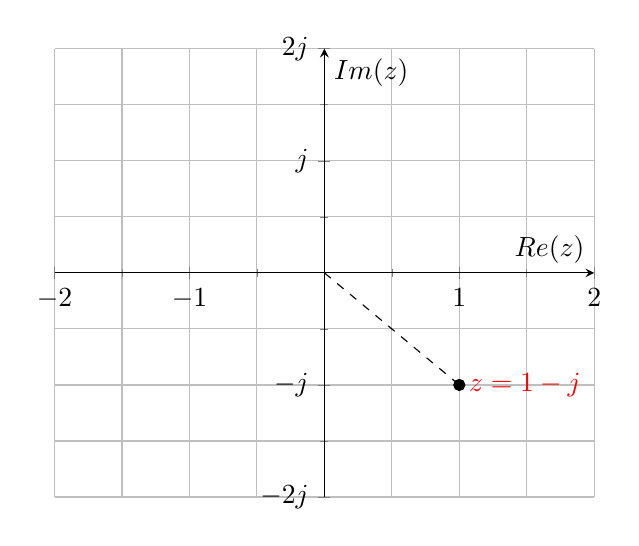
\begin{tikzpicture}

\begin{axis}
    [
    ytick ={-3,...,4}, yticklabels={$-3j$, $-2j$, $-j$, $0$, $j$, $2j$, $3j$, $+3j$, $+4j$},
    axis lines = center,
    grid=both,
    minor tick num=1,
    ticks=both,
    xlabel=$Re(z)$,
    ylabel=$Im(z)$,
    ymin=-2,
    ymax=+2,
    xmin=-2,
    xmax=+2
    ]

    \addplot [black, mark = *] coordinates {( 1, -1)} {};
    
    \node [right, red] at (axis cs:  1, -1) {$z = 1-j$};
    

    \addplot [dashed, black] coordinates { (0,0) (1,-1) };

\end{axis}
\end{tikzpicture}
    
    \item %write the solution of q2b
    Given \ $z = re^{j\theta}$ \ and \ $z^4 = -81$ \\
    \\
    $z^4 = r^4 e^{4j\theta} = -81$ \\
    $r^4 (\cos(4\theta) + j\sin(4\theta)) = -81$ \\
    \\
    Here, we have only real $-81$ at the right hand side of the equation. For this reason, left hand side should also be real. \\
     Therefore, $j\sin(4\theta) = 0$. \\
     Therefore, \\
      $4\theta = 0$ \ , i.e. $\theta = 0$  \ or \\
       $4\theta = \pi$ \ , i.e. $\theta = \frac{\pi}{4}$\\
       \\
      \underline{First case:} If we put $\theta = 0$ to our equation: \\
      $r^4 (\cos(0) + j\sin(0)) = -81$ \\
      $r^4(1+0) = -81$ \\
      $r^4 = -81$ \ Since r(magnitude) must be a real value, there can not be a real number such that its fourth power is equal to negative number. Therefore, we could not reach the solution. \\
      \\
       \underline{Second case:} If we put $\theta = \frac{\pi}{4}$ to our equation: \\
      $r^4 (\cos(4\frac{\pi}{4}) + j\sin(4\frac{\pi}{4})) = -81$ \\
      $r^4(-1+0) = -81$ \\
      $-r^4 = -81$ \\
      $r^4 = 81$ \\
      $r = 3$ \ Now, we get the real value for r(magnitude). Therefore our complex number $z$ is: \\
      $z = 3e^{j\frac{\pi}{4}}$ \ [RESULT]
    \item %write the solution of q2c
    $z = \frac{(\frac{1}{2} + \frac{1}{2}j)(1-j)}{1- \sqrt{3}j} = \frac{\frac{1}{2} + \frac{-j}{2} + \frac{j}{2} - \frac{1}{2}j^2}{1- \sqrt{3}j} = \frac{1}{1- \sqrt{3}j}$ \\
    \\
    if we multiply both numerator and denominator of $z$ with conjugate of $1- \sqrt{3}j$ (which is equal to $1 + \sqrt{3}j$): \\
    \\
    $z = \frac{1 + \sqrt{3}j}{(1 + \sqrt{3}j)(1 - \sqrt{3}j)} = \frac{1 + \sqrt{3}j}{1 -\sqrt{3}j + \sqrt{3}j - 3j^2} = \frac{1 + \sqrt{3}j}{4}$ \\
    \\
    Hence, \ $z = \frac{1 + \sqrt{3}j}{4}$ \\
    \\
    \underline{For magnitude:} $|z| = \sqrt{(\frac{1}{4})^2 + (\frac{\sqrt{3}}{4})^2} = \sqrt{\frac{1}{16} + \frac{3}{16}} = \sqrt{\frac{4}{16}} = \sqrt{\frac{1}{4}} = \frac{1}{2} $ \\
    \\
    \underline{For angle:} We know that $ \theta = \taninv(\frac{b}{a})$ for $z = a +bj$ \\
    Therefore, $\theta = \taninv(\frac{\frac{\sqrt{3}}{4}}{\frac{1}{4}}) = \taninv(\sqrt{3}) = \frac{\pi}{3}$ \\
    Therefore, magnitude is: $|z| = \frac{1}{2}$ \ and \ angle is: $\theta = \frac{\pi}{3}$ \ [RESULT]
    
    \item %write the solution of q2d
    $z = -\frac{3}{j}e^{j\frac{\pi}{2}}$  \\
    Let's say $z = z_1z_2$ \ , \ $z_1 = -\frac{3}{j}$ \ and \ $z_2 = e^{j\frac{\pi}{2}}$\\
    First, we need to convert $z_1 = -\frac{3}{j}$ to polar form. \\
    $z_1 = \frac{-3}{j}$, multiply numerator and denominator with conjugate of denominator which is $-j$. \\
    $\frac{(-3)(-j)}{(j)(-j)} = \frac{3j}{-j^2} = 3j$ \\
    \\
    When we plot $z_1 = 3j$ on the complex plane: \\
    
    \begin{figure}[h]
\centering
\begin{tikzpicture}[scale=1]
 \begin{scope}[thick,font=\scriptsize]
    \draw [->] (-.5,0) -- (5.5,0) node [above left]  {$\operatorname{Re} $};
    \draw [->] (0,-.5) -- (0,4) node [below right] {$\operatorname{Im} $};
  \end{scope}
  \coordinate (o) at (0,0);
  \coordinate (z) at (0,3);
  \coordinate (zx) at (4,0);
  \coordinate (zy) at (0,3);
  
  \draw[ultra thick,red]  (0,0) --  (z) node [right] {$3j$};
  
  \pic[draw, "$\theta = \frac{\pi}{2}$", ->, angle eccentricity=0.8,angle radius = 1.5cm] {angle = zx--o--z}; 
\end{tikzpicture}

\end{figure}

	We see that magnitude of $z_1$ is equal to $r=3$ and angle of $z_1$ is $\theta = \frac{\pi}{2}$. \\
	Therefore, polar form of $z_1$ is equal to: \\
	$z_1 = 3e^{j\frac{\pi}{2}}$ \\
	\\
	Our $z_2 = e^{j\frac{\pi}{2}}$ was already in polar form. \\
	Therefore, when we put these values on given equation: \\
	$z = z_1z_2$ \\
	$z = 3e^{j\frac{\pi}{2}}e^{j\frac{\pi}{2}}$ \\
	$z = 3e^{j\pi}$ [RESULT] \\
	\\
	
    
    \end{enumerate}

\item %write the solution of q3  
$y(t) = 2x(\frac{1}{2}t + 3)$
\begin{figure}[h!]
    \centering
        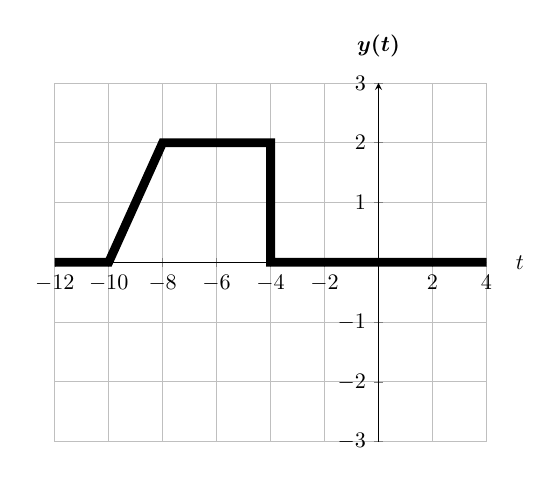
\begin{tikzpicture}[scale=0.8]
           \begin{axis}[
          axis lines=middle,
          xlabel={$t$},
          ylabel={$\boldsymbol{y(t)}$},
          xtick={-12, -10, -8, -6, -4, -2, ..., 4},
          ytick={-3, -2, -1, ..., 3},
          ymin=-3, ymax=3,
          xmin=-12, xmax=4,
          every axis x label/.style={at={(ticklabel* cs:1.05)}, anchor=west,},
          every axis y label/.style={at={(ticklabel* cs:1.05)}, anchor=south,},
          grid,
        ]
           \path[draw,line width=4pt] (-12,0) -- (-11,0) -- (-10,0) -- (-8,2) -- (-4,2) -- (-4,0) -- (3,0) -- (4,0);
           \end{axis}
        \end{tikzpicture}
        \caption{$t$ vs. $y(t)$.}
        \label{fig:q3}
    \end{figure}

\item %write the solution of q4
    \begin{enumerate}
    % Write your solutions in the following items.
    \item %write the solution of q4a
    Firstly, we need to find $x[-n]$: \\
    
    \begin{figure} [h!]
    \centering
    \begin{tikzpicture}[scale=0.9] 
      \begin{axis}[
          axis lines=middle,
          xlabel={$n$},
          ylabel={$\boldsymbol{x[-n]}$},
          xtick={ -7, -6, -5, -4, -3, -2, -1, 0, 1,2,3,4,5,6,7},
          ytick={-4, -3, -2, -1, ..., 4},
          ymin=-4, ymax=4,
          xmin=-7, xmax=7,
          every axis x label/.style={at={(ticklabel* cs:1.05)}, anchor=west,},
          every axis y label/.style={at={(ticklabel* cs:1.05)}, anchor=south,},
          grid,
        ]
        \addplot [ycomb, black, thick, mark=*] table [x={n}, y={xn}] {q4a_1.dat};
      \end{axis}
    \end{tikzpicture}
    \caption{$n$ vs. $x[-n]$.}
    \label{fig:q4}
\end{figure}
	
	Secondly, we need to find $x[2n+1]$: \\
    
    \begin{figure} [h!]
    \centering
    \begin{tikzpicture}[scale=0.8] 
      \begin{axis}[
          axis lines=middle,
          xlabel={$n$},
          ylabel={$\boldsymbol{x[2n+1]}$},
          xtick={ -1, 0, 1, 2, 3,4,5,6,7},
          ytick={-4, -3, -2, -1, ..., 4},
          ymin=-4, ymax=4,
          xmin=-1, xmax=7,
          every axis x label/.style={at={(ticklabel* cs:1.05)}, anchor=west,},
          every axis y label/.style={at={(ticklabel* cs:1.05)}, anchor=south,},
          grid,
        ]
        \addplot [ycomb, black, thick, mark=*] table [x={n}, y={xn}] {q4a_2.dat};
      \end{axis}
    \end{tikzpicture}
    \caption{$n$ vs. $x[2n+1]$.}
    \label{fig:q4}
\end{figure}


RESULT is $x[-n] + x[2n+1]$: \\
    
    \begin{figure} [h!]
    \centering
    \begin{tikzpicture}[scale=1.0] 
      \begin{axis}[
          axis lines=middle,
          xlabel={$n$},
          ylabel={$\boldsymbol{x[-n] + x[2n+1]}$},
          xtick={ -7,-6,-5,-4,-3,-2,-1, 0, 1, 2, 3,4,5,6,7},
          ytick={-4, -3, -2, -1, ..., 4},
          ymin=-4, ymax=4,
          xmin=-7, xmax=7,
          every axis x label/.style={at={(ticklabel* cs:1.05)}, anchor=west,},
          every axis y label/.style={at={(ticklabel* cs:1.05)}, anchor=south,},
          grid,
        ]
        \addplot [ycomb, black, thick, mark=*] table [x={n}, y={xn}] {q4a_3.dat};
      \end{axis}
    \end{tikzpicture}
    \caption{$n$ vs. $x[-n] + x[2n+1]$.}
    \label{fig:q4}
\end{figure}
    
    \item %write the solution of q4b
    
    $x[-n] + x[2n+1] = -4\delta[n+7] + 3\delta[n+4] -2\delta[n+2] + \delta[n+1] + \delta[n-1] -4\delta[n-3]$
    \end{enumerate}

\item %write the solution of q5
    \begin{enumerate}
    % Write your solutions in the following items.
    \item %write the solution of q5a
    
    We know that $\cos(t)$ is a periodic function with fundamental period $T_0 = 2\pi$.\\
     For given signal $x(t) = 3 \cos(7\pi t - \frac{4\pi}{5})$: \\
     \begin{itemize}
  	\item Coefficient 3 just determines amplitude, it does not affect period.
  	\item $-\frac{4 \pi}{5}$ is just time-shift and it also does not affect period of cosine.
  	\item $7 \pi$ which is coefficient of t is time-scale and it affects period of cosine. 
	\end{itemize}
	
	Thus, given signal is periodic with fundamental period $T_0 = \frac{2 \pi}{7 \pi} = \frac{2}{7}$ 
    \item %write the solution of q5b
    
    We know that discrete time signal $\sin[wn]$ is periodic with fundamental period $N_0 = \frac{2 \pi}{w}k$  \\ for possible minimum $ k \in \mathbb{Z}^+$ which makes $N_0 \in \mathbb{Z}^+$ also. \\
    Therefore, for given discrete time signal $\sin[4n - \frac{\pi}{2}]$: \\
    \\
    $N_0 = \frac{2 \pi}{4} k$ \\
    Here, since $\pi$ is irrational number, there is no any $k \in \mathbb{Z}^+$ which makes $N_0$ integer. \\
    Therefore, given discrete time signal is \textbf{not periodic}.
    \item %write the solution of q5c
    
    For $2 \cos[\frac{7 \pi}{5}n]$, \ fundamental period $N_0 = \frac{2 \pi}{\frac{7 \pi}{5}} k$ \ such that $k$ should be minimum possible positive integer that makes $N_0 \in \mathbb{Z}^+$ also. \\
    \\
    Therefore, $N_0 = \frac{2 \pi}{\frac{7 \pi}{5}} k = 2 \pi \frac{5}{7 \pi} k = \frac{10}{7} k $ \\
    When $k=7$, \ $N_0 = 10$ \\
    \\
    \\
    For $7 \sin[\frac{5 \pi}{2}n - \frac{\pi}{3}]$, again according to above definition: \\
    \\
    $N_0 = \frac{2 \pi}{\frac{5 \pi}{2}} k = 2 \pi \frac{2}{5 \pi} k  = \frac{4}{5} k $ \\
    When $k=5$, \ $N_0 = 4$ \\
    \\
    As a result, for given signal in the question $x[n] = 2 \cos[\frac{7 \pi}{5}n] + 7 \sin[\frac{5 \pi}{2}n - \frac{\pi}{3}]$: \\
    We need to find least common multiple of periods of these two signals which is equal to: \\
    LCM(10,4) = 20 \\
    Thus, given signal is periodic with period $N=20$. 
    \end{enumerate}


\item %write the solution of q6
    \begin{enumerate}
    % Write your solutions in the following items.
    \item %write the solution of q6a
    We know that the signal is even if $x(t) = x(-t)$. When we look at the given figure: \\
     For $-2 < t < -1$, \ outputs are: $0 < x(t) < 1$ \\
     However, for $1 < -t < 2$, \ outputs are: $x(-t) = 0$. This contradicts to above statement. \\
     In other words, for this region of inputs, the signal is not symmetric with respect to y axis. Therefore, this is a contradiction and given signal is not even.\\
     \\
     We know that the signal is odd if $x(t) = -x(-t)$. When we look at the given figure: \\
     $x(1) = 1$, \ and \ $-x(-1) = -1$. They are not equal to each other. This is a contradiction to above statement. Thus, this signal is not odd. 
    \item %write the solution of q6b
    
    We know that $Even \{x(t)\} = \frac{1}{2}(x(t) + x(-t))$  \ and \ $Odd \{x(t)\} = \frac{1}{2}(x(t) - x(-t))$ \\
  \[x(t) = \begin{cases} 
      0 & t < -2 \\
      t+2 & -2\leq t < -1 \\
      1 & -1 \leq t \leq 1 \\
      0 & 1<t 
   \end{cases}
\]

\[x(-t) = \begin{cases}
	  0 & t < -1 \\ 
	  1 & -1\leq t \leq 1 \\
	  -t+2 & 1 < t \leq 2 \\
	  0 & 2<t  
   \end{cases}
\]
\\
According to above definitions: \\
\[Even \{x(t)\} = \frac{1}{2}(x(t) + x(-t)) =  \begin{cases}
	  0 & t<-2  \\
	  \frac{t+2}{2} & -2 \leq t < -1 \\
	  1 & -1\leq t \leq 1 \\
      \frac{-t+2}{2} & 1 < t \leq 2 \\
      0 & 2 < t 
   \end{cases}
\]

\[Odd \{x(t)\} = \frac{1}{2}(x(t) - x(-t)) =  \begin{cases}
	  0 & t<-2  \\
	  \frac{t+2}{2} & -2 \leq t < -1 \\
	  0 & -1\leq t \leq 1 \\
      \frac{t-2}{2} & 1 < t \leq 2 \\
      0 & 2 < t 
   \end{cases}
\]
\\

\begin{figure}[h!]
    \centering
        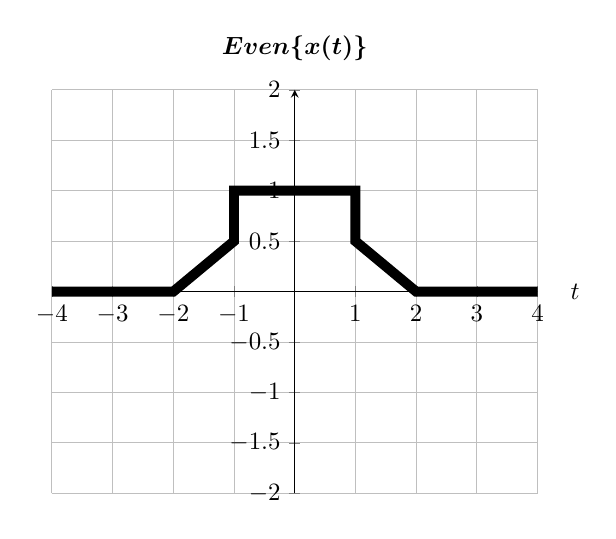
\begin{tikzpicture}[scale=0.9]
           \begin{axis}[
          axis lines=middle,
          xlabel={$t$},
          ylabel={$\boldsymbol{Even\{x(t)\}}$},
          xtick={-4, -3, -2, -1, 0, 1, ..., 4},
          ytick={-2, -1.5, -1, -0.5, 0, 0.5, 1 ,1.5, 2},
          ymin=-2, ymax=2,
          xmin=-4, xmax=4,
          every axis x label/.style={at={(ticklabel* cs:1.05)}, anchor=west,},
          every axis y label/.style={at={(ticklabel* cs:1.05)}, anchor=south,},
          grid,
        ]
           \path[draw,line width=4pt] (-4,0) -- (-2,0) -- (-1,0.5) -- (-1,1) -- (1,1) -- (1,0.5) -- (2,0) -- (4,0);
           \end{axis}
        \end{tikzpicture}
        \caption{$t$ vs. $Even\{x(t)\}$.}
        \label{fig:q6_1}
    \end{figure}
    
    \begin{figure}[h!]
    \centering
        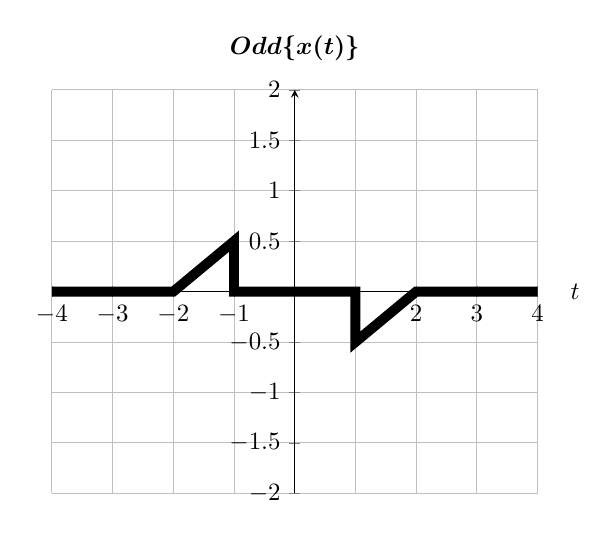
\begin{tikzpicture}[scale=0.9]
           \begin{axis}[
          axis lines=middle,
          xlabel={$t$},
          ylabel={$\boldsymbol{Odd\{x(t)\}}$},
          xtick={-4, -3, -2, -1, 0, 1, ..., 4},
          ytick={-2, -1.5, -1, -0.5, 0, 0.5, 1 ,1.5, 2},
          ymin=-2, ymax=2,
          xmin=-4, xmax=4,
          every axis x label/.style={at={(ticklabel* cs:1.05)}, anchor=west,},
          every axis y label/.style={at={(ticklabel* cs:1.05)}, anchor=south,},
          grid,
        ]
           \path[draw,line width=4pt] (-4,0) -- (-2,0) -- (-1,0.5) -- (-1,0) -- (1,0) -- (1,-0.5) -- (2,0) -- (4,0);
           \end{axis}
        \end{tikzpicture}
        \caption{$t$ vs. $Odd\{x(t)\}$.}
        \label{fig:q6_2}
    \end{figure}
    
    \end{enumerate}

\item %write the solution of q7
    \begin{enumerate}
    % Write your solutions in the following items.
    \item %write the solution of q7a
    $x(t) = -3u(t-2) + 5u(t-3) -3u(t-5)$ \\
    \item %write the solution of q7b
    $\frac{dx(t)}{dt} = -3 \frac{du(t-2)}{dt} +5 \frac{du(t-3)}{dt} -3 \frac{du(t-5)}{dt}$ \\
    \\
    $\frac{dx(t)}{dt} = -3 \delta(t-2) +5 \delta(t-3) -3 \delta(t-5)$
    
    \begin{figure} [h!]
    \centering
    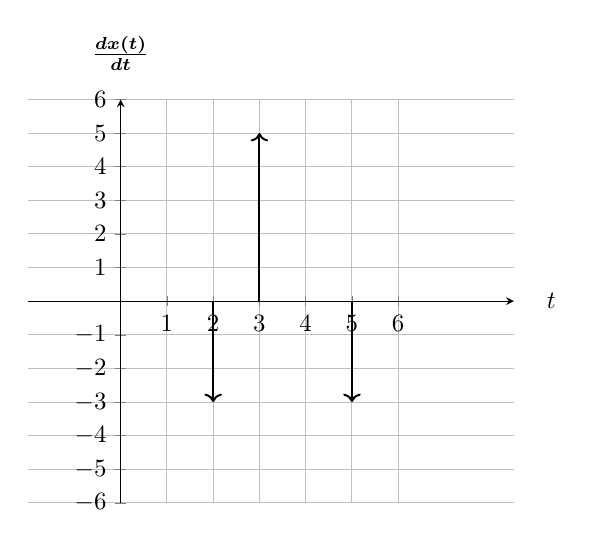
\begin{tikzpicture}[scale=0.9] 
      \begin{axis}[
          axis lines=middle,
          xlabel={$t$},
          ylabel={$\boldsymbol{\frac{dx(t)}{dt}}$},
          xtick={0, 1, ..., 6},
          ytick={-6, -5, -4, -3, -2, -1, 0, 1, 2, 3, 4, 5, 6},
          ymin=-6, ymax=6,
          xmin=-2, xmax=8.5,
          every axis x label/.style={at={(ticklabel* cs:1.05)}, anchor=west,},
          every axis y label/.style={at={(ticklabel* cs:1.05)}, anchor=south,},
          grid,
        ]
        
        \addplot [black, thick, ->] coordinates {(2,0) (2,-3)};
        \addplot [black, thick, ->] coordinates {(3,0) (3,5)};
        \addplot [black, thick, ->] coordinates {(5,0) (5,-3)};
      \end{axis}
    \end{tikzpicture}
    \caption{$t$ vs. $\frac{dx(t)}{dt}$.}
    \label{fig:q7}
\end{figure}
    
   
    \end{enumerate}    

\item %write the solution of q8
    \begin{enumerate}
    % Write your solutions in the following items.
    \item %write the solution of q8a
    \begin{itemize}
  	\item The system has memory because current output depends on past value of input. For example, for $n = 1$: \\
  	$y[1] = x[3 \times 1 -5] = x[-2]$ \ (Output at $n=1$ depends on past input at $n=-2$)
  	\item The system is stable because when we choose input signal as bounded signal such as unit step function, outputs will also be bounded.
  	\item The system is \textbf{not} causal because for some outputs, output depends on future value of input. For example, for $n=4$: \\
  	 $y[4] = x[3 \times 4 -5] = x[7]$ \ (Output at $n=4$ depends on future input at $n=7$, and this contradicts to causality principle)
  	 \item 	The system is not time invariant. \\
  	  Definition of time-invariance is: $y[n-n_0] = h[x[n - n_0]]$ \\
  	  $=>x_1[n]=>x[n-n_0]\\
  	   =>y_1[n] = x_1[3n-5]\\
  	   =>y_1[n]=x[3n-n_0-5]\\ 
  	   =>y_1'[n]=y[n-n_0]\\
  	   =>y_1'[n]=x[3(n-n_0)-5]\\
  	   =>y_1'[n]=x[3n-3n_0-5]\\
  	   y_1' \neq y_1
  	   $ \\
  	   Thus, this system is not time-invariant.
  	 \item The system is invertible,we can find inverse of h\\
  	 $y[n] = h[x[3n - 5]]\\
  	 x[n]= h^{-1}[y[(n+5)/3]]$
  	 \item The system is linear if superposition property hold\\
  	 $y[n]=x[3n-5]\\
  	 y_1[n]=x_1[3n-5]\\
  	 y_2[n]=x_2[3n-5]\\
  	 x_3=a_1 \times x_1 + a_2 \times x_2 \\
  	 y_3=x_3[3n-5]\\
  	 y_3=a_1\times x_1[3n-5]+a_2 \times x_2[3n-5]\\
  	 y_3' = a_1 \times y_1+a_2 \times y_2\\
  	 y_3=y_3' $
  	 This system is linear
  	 
	\end{itemize}
    \item %write the solution of q8b
    \begin{itemize}
    \item The system has memory because current output depends on past value of input. For example, for $n = 1$: \\
  	$y(1) = x(3 \times 1 -5) = x(-2)$ \ (Output at $n=1$ depends on past input at $n=-2$)
  	\item The system is stable because when we choose input signal as bounded signal, outputs will also be bounded.
  	\item The system is \textbf{not} causal because for some outputs, output depends on future value of input. For example, for $n=4$: \\
  	 $y(4) = (3 \times 4 -5) = x(7)$ \ (Output at $n=4$ depends on future input at $n=7$, and this contradicts to causality principle)
  	 \item	The system is not time invariant. \\
  	  Definition of time-invariance is: $y[t-t_0] = h[x[t - t_0]]$ \\ $ =>x_1(t)=>x(t-t_0)\\
  	   =>y_1(t) = x_1(3t-5)\\
  	   =>y_1(t)=x(3t-t_0-5)\\ 
  	   =>y_1'(t)=y(t-t_0)\\
  	   =>y_1'(t)=x(3(t-t_0)-5)\\
  	   =>y_1'(t)=x(3t-3t_0-5)\\
  	   y_1' \neq y_1
  	   $ \\
  	   Thus, this system is not time-invariant.
  	 \item The system is  invertible,we can try find inverse of h\\
  	 $y(t) = h(x(3t - 5))\\
  	 x(t)= h^{-1}(y((t+5)/3))$\\
  	 The system is invertible.
  	   	 \item The system is linear if superposition property hold\\
  	 $y(n)=x(3n-5)\\
  	 y_1(n)=x_1(3n-5)\\
  	 y_2(n)=x_2(3n-5)\\
  	 x_3=a_1 \times x_1 + a_2 \times x_2 \\
  	 y_3=x_3(3n-5)\\
  	 y_3=a_1\times x_1(3n-5)+a_2 \times x_2(3n-5)\\
  	 y_3' = a_1 \times y_1+a_2 \times y_2\\
  	 y_3=y_3' $
  	 This system is linear
  	 \end{itemize}

    \item %write the solution of q8c
    \begin{itemize}
    \item The system has memory because\\ $y(t)=tx(t-1)$. For $t=1\\ y(t)=1x(0)$ we need past value of x
    \item The system is causal, we do not need any future value of x.
    \item $y(t) = h(tx(t-1))\\
    x(t) = h^{-1}(y(t+1)/(t+1))$\\we can find invertible of h.The system is invertible.
    \item The system is not time invariant\\ $y(t) = tx(t-1)\\
    y'(t)= y(t-t0) = (t-t0) \times x(t-t0-1)\\
    x_1(t)=x(t-t0-1)\\
    y(t) = t \times x_1(t) = t \times (t-t0-1) \\
    y(t)  \neq y'(t) $  \\
    Thus, the system is not time-invariant.
    \item The system is linear if superposition property hold\\ $y(t)=x(t-1)\times t \\ 
  	 y_1(t) => t \times x_1(t-1)  \\
  	 y_2(t) => t \times x_2(t-1) \\ 
  	 x_3= a_1 \times x_1 + a_2 \times x_2\\
  	 y_3=x_3 \times t \\
  	 y_3= t \times(a_1 \times x_1 + a_2 \times x_2)=a_1 \times y_1 + a_2 \times y_2\\
  	 t \times (a_1 \times x_1(t-1) + a_2 \times x_2(t-1))= a_1 \times t  \times x_1(t-1) + a_2 \times t \times x_2(t-1)$\\
  	 The system is linear
  	 \item The system is not stable \\
  	 $y(t) = tx(t-1)\\
  	 y(t)/t =x(t-1)$ If t=0 \\
  	 $y(0)/0 = x(-1)$ \\
  	 Output is $\infty$ for $x(-1)$. Thus, output signal is unbounded and system is not stable.
    \end{itemize}

    \item %write the solution of q8d
    \begin{itemize}
    \item The system has memory.\\
    $k=1 => x[n-1]\\
    k=2 => x[n-2]$. It continues like this in the summation. Thus, we need past values of inputs.
    \item The system is casual because we do not need any future inputs. The system depends only the past inputs.
    \item The system is not stable. Even if all inputs are bounded and their summation can also be bounded,the output goes towards infinity since k's upper limit is also infinity, so output is not bounded.
    \item The system is invertible.\\$y[n+1]=x[n]+x[n-1]+x[n-2]+...\\
    y[n]=x[n-1]+x[n-2]+...\\
    y[n+1]-y[n]=x[n]$ \\
    As you see, we can reach $x[n]$ again. Thus, the system is invertible.
    \item The system is time invariant\\
    $x_1[n]= x[n-n_0]\\
    y[n]=x_1[n]\\
    y[n]= \sum_{k=1}^{\infty} x[n-n_0-k] \\
    y'[n]=y[n-n_0]\\
    y'[n]=\sum_{k=1}^{\infty} x[n-n_0-k]\\
    y[n]=y'[n]$
    \item As we explained in previous items, the sytsem is linear if superposition property hold.\\
    $y_1[n]=\sum_{k=1}^{\infty} x_1[n-k]\\
    y_2[n]=\sum_{k=1}^{\infty} x_2[n-k]\\
    y_3[n]=a_1y_1[n] + a_2y_2[n]\\
    x_3[n]=a_1x_1[n]+a_2x_2[n]\\
    y_3'[n]= \sum_{k=1}^{\infty} x_3[n-k]\\
    y_3'[n]=a_1 \sum_{k=1}^{\infty} x_1[n-k] + a_2 \sum_{k=1}^{\infty} x_2[n-k]\\
    y_3[n]=y_3'[n]$ \\
    Thus, the system is linear.
    
    
    \end{itemize}
    \end{enumerate}
    
\end{enumerate}
\end{document}

